\documentclass{article}
\usepackage{array}
\usepackage{hyperref}
\usepackage {graphicx}
\usepackage{longtable}
\usepackage{url}

\usepackage[toc,page]{appendix}

\title{Introduction to GenAMap}

\setlength\parindent{0pt}

\author{}
\date{}

\begin{document}

\maketitle

\tableofcontents
\vspace{1cm}
For further questions / comments / suggestions, please contact \url{genamapsupport@cs.cmu.edu}

\section{What is GenAMap?}

GenAMap is software for association mapping and eQTL- and genome-wide association studies. It combines automated data analysis and rich visual exploration tools to enable users to perform an association study end-to-end within a single platform. Once users have imported genome data, transcriptome data and / or phenotypic trait data into GenAMap, they can deploy a variety of methods for analysis, both classical test-based methods such as the wald test and modern structured regression algorithms such as the GFLasso. The results produced can then be explored directly within the software using a range of visualization tools that are designed to enable the user to gain an overview of a potentially large amount of result data, spot interesting patterns easily and then drill down into those patterns and request details. In this way, GenAMap enables users to gain a quality of insight that is difficult to achieve using either machines alone or by database queries.\\

GenAMap offers the following advantages: 

\begin{itemize}
\item A range of sophisticated algorithms at the users disposal that can be started with a few clicks from a graphical interface. 
\item Automatic delegation of algorithm computation to a remote computer cluster. This frees the user from having to provide high-performance hardware and enables him or her to run algorithms on even large data sets in a timely manner.
\item Customized visualization tools that both scale to large datasets and allow the user to discover and explore nuances. 
\item Results are ready for visualization immediately as an algorithm finishes running. The user does not need to reformat data or port information between different stand-alone tools.
\item Graphs produced within GenAMap are high-quality and can be embedded in publications.
\end{itemize}

This tutorial is structured as follows: In section \ref{example}, we will introduce the reader to the GenAMap interface using an example. In section \ref{coreFeatures}, we describe the core features of GenAMap in detail. In section \ref{architecture}, we outline the technical architecture underlying GenAMap and describe GenAMap's technical capabilities, limitations and system requirements. Finally, in section \ref{furtherFeatures}, we describe further features in GenAMap.\\

Throughout this tutorial, I will be referring to the video tutorials that can be accessed via the GenAMap website \ref{videos}. Please visit \url{http://sailing.cs.cmu.edu/genamap/tutorials.html}. In addition to online resources, further documentation comes packaged with GenAMap. In the `Documentation' folder, you can find the following tutorials:

\begin{itemize}
\item `SettingUpGenAMap.pdf' guides you through the installation, registration and login process.
\item `DataImportingGuide.pdf' shows you how to format data for importing into GenAMap. We also provide examples of correctly formatted data in the `ExampleData' subfolder.
\item `AlgorithmsGuide.pdf' provides details on each of the algorithms available in GenAMap, together with information about their implementation.
\end{itemize}

Please note that GenAMap is a software under development. As such, bugs / non-availabilities of functions will occur from time to time. If GenAMap is not behaving as expected for your, please first restart the software. If the same problem keeps coming up, please contact the developers under \url{genamapsupport@cs.cmu.edu}




\section{A first example} \label{example}

In this section, we will give a flavor of the GenAMap interface using a simple example. Given synthetic marker data (marker = SNP) and phenotypic trait data, we would like to find associations between individual markers and traits using the Lasso algorithm. We assume that GenAMap is already set up on the users machine and is ready for use. To learn more about this initial setup, please refer to `SettingUpGenAMap.pdf' in the Documentation folder. The data used in this section is available in `Documentation/ExampleData'. Using this data, you can perform the same steps as described here.\\

After logging in for the first time using a fresh user account, the interface presents itself as in Figure \ref{blank}. The first thing we need to do is add a project. A project is similar to a folder, used to organize a data collection. We right-click on the `Projects' field in the top left and choose `Add new Project'. This brings up the project creation dialog box as in Figure \ref{projCreate}. We type in the name `GenAMapTutorial' and click on `Create'. Now, the project appears as a sub-item under `Projects' in the top left corner.\\

\paragraph{Data Importing} Once the project has been created, we can import the marker data. Right-click on the newly created project, choose `Add Marker Data' and fill out the appearing marker import dialog. We would like to add this data to our project `GenAMapTutorial'. Select this project in the drop-down menu at the top if it is not already selected. Then, we give our Marker Data set a name. We choose `firstMarkerSet'. The dialog requires us to specify three files: A file containing the actual marker values, a file containing the labels of the markers and a file containing the labels of the samples. We choose the following files from the `ExampleData' folder: `markerVals.txt', `markerLabelsReal.txt' and `sampleLabels.txt'. For more information on the formatting of these files and how to format your own data, please refer to `DataImportingGuide.pdf'. Also, using the example data provided, we can ignore the formatting options at the bottom of the dialog. The completed marker import dialog is shown in Figure \ref{markerImport}. \\

Now, we click on the `Import' button. This will open up a separate window as in Figure \ref{importBar} that displays a progress bar that indicates what proportion of the import has (approximately) been completed. This window is used to keep the user updated on many potentially time-intensive data operations. While the marker data is being imported, the user is free to use any other feature available in GenAMap. For more information on marker importing, view `Importing markers tutorial' (see Appendix \ref{videos}).\\

Once the marker data is imported, the data set is visible under our project in the Marker Tab as shown in Figure \ref{markerTab}. When we click on the Marker Data set, the chromosome browser appears at the bottom of the screen, as in Figure \ref{chromBrowser}. This is one of our visualization tools. It allows us to view the location of individual markers along the chromosome. The green dots represent markers or groups of markers. For more information on using the chromosome browser, view `Exploring and selecting markers tutorial' (see Appendix \ref{videos}).\\

Now it is time to import the phenotypic trait data. We right-click on our project and select `Add Trait Data'. This opens up the trait importing dialog. We fill out this dialog exactly as before, providing files `geneVals.txt', `geneLabels.txt' and `sampleLabels.txt'. Again, we can ignore the formatting options at the bottom. For more information on trait file formatting, please refer to `DataImportingGuide.pdf'. The completed trait import dialog is shown in Figure \ref{traitImport}. For more information on trait importing, please refer to `Importing traits tutorial' (see Appendix \ref{videos}). When the trait data has finished importing, we can see it under our project when we browse to the Trait Tab in the data management section of the interface, as shown in Figure \ref{traitTab}. \\

\paragraph{Running the Lasso} At this time, we have all the information we need (Marker Data and Trait Data) to tun the Lasso algorithm to find associations between individual markers and traits. Right-click on the project and then click on `Add Association Data'. This brings up the Association Data creation box. There, we have the option to choose between importing Association Data that has been computed externally or to run an algorithm to compute a new data set. First, we choose the name of our project from the drop down menu at the top. Below that, we select the two data sets we uploaded as input data for our algorithm. Next, we select a name for our Association Data set. We choose `lassoAssocs'. As we want to use Lasso to create the algorithm, we select the radio button `Create a new Association' and `Lasso' under the `Algorithm' drop down menu. Now, we are ready to click `Run'. The filled out Association Data creation dialog box is shown in Figure \ref{assocCreation}. For more information on creating Association Data, please refer to `Running association algorithms tutorial' (see Appendix \ref{videos}). \\

Once the Lasso begins executing, two status bars will appear in the bottom left corner of the screen as shown in \ref{controlCenter}. This area is called the `Algorithm Control Center'. The Lasso is executed on a remote computer cluster. The cluster communicates with the local instance of GenAMap about the status of the algorithm. Note that it is not necessary to leave GenAMap or even your local computer running while Lasso is executing. You can shut down your machine and the results will most likely be immediately available upon restart. When the status bar reaches 100\%, the results will be ready for visualization or further processing. Note that there are two status bars because GenAMap also computes a Trait Network at the same time to enrich the association visualization later. For more information about user options in the Algorithm Control Center, view `Using the algorithm control center tutorial' (see Appendix \ref{videos}). Once the Lasso algorithm has finished, the data is downloaded from the remote cluster to your local machine. You can see it if you navigate to the Association Tab in the top left of the screen as shown in figure \ref{assocTab}. \\

\paragraph{Visualizing the results} We click on the Association Data set and the matrix view will appear, as in figure \ref{matrixView}. This is a graphical representation of the computed association values. The markers are plotted on the y-axis and the traits are plotted on the x-axis. Dark pixels correspond to non-zero associations. The pattern that appears is somewhat chaotic. However, we can see that the dots form a kind of grid shape, which indicates that some traits are associated with many markers and some markers are associated with many traits. \\

To reveal the structure in the data, we would like to visually group traits together that are associated to similar markers. Right now, the traits and markers are ordered as they were in the files that were used for importing (which was a random order). To change this order, we need to create a `Clustering'. `Clustering' is GenAMap's name for data that captures order information among traits. We right-click in the matrix view and choose `Add Cluster'. This brings up the Clustering creation dialog. We fill in the name of our project and Trait Data set at the top, choose a name for the Clustering itself and click the radio button `Create a new Clustering'. We pick the only available choices in the `Algorithm' and `Network' drop down menus and hit `Run'. The filled out dialog is shown in Figure \ref{clusterCreation}. The Clustering Algorithm completes in the same way as Lasso. Once the Clustering is available, we can right-click in the Matrix View and select `Set Clustering'. Now the traits are re-ordered according to the Clustering as in Figure \ref{matrixViewClustered}. This immediately confirms our hypothesis that a small set of traits is associated with several markers. We find that markers are associated with blocks of traits. Within these blocks, traits have a highly similar association profile. We can zoom into the interesting region by selecting it with the mouse, as shown in Figure \ref{matrixViewZoomed}. To learn more about the matrix view, please view `How to use GenAMap's matrix view tutorial' (see Appendix \ref{videos}).\\

We expect that traits with similar association profiles are highly related. To confirm this hypothesis, we right-click in the visualization area and select `Switch to JUNG view'. Now we see the traits in a ball-and-stick representation called the JUNG view, as shown in Figure \ref{JUNG}. Lines between traits indicate relatedness. We can use the mouse to drag around the traits on the screen and find that they indeed form distinct groups as shown in Figure \ref{JUNGgrouped}. The labels next to the nodes tell us which traits belong to these groups. To compare the association profiles of the traits in one of these groups in detail, we select all traits in the group, right-click on one of the traits and then choose `View Manhatten Plot'. This brings up the Manhatten plot (as in Figure \ref{manhattan}) which shows the association strengths of the traits in the group we have selected against the genome. We find that all traits have highly similar association strengths towards several markers on chromosome 2. To learn more about the JUNG View and Manhatten Plot, please view `Network visualization using the JUNG view tutorial' / `Manhatten plots tutorial' respectively (see Appendix \ref{videos}). \\

In this section, we provided a snapshot of the capabilities of GenAMap. We imported marker and trait data, ran the Lasso algorithm and explored the results. In the following chapters, we will give a systematic account of these and further features available in GenAMap.




\section{Core Features}  \label{coreFeatures}

\paragraph{Overview of GenAMap} GenAMap roughly supports three kinds of user actions: importing data, running algorithms and visualizing data. Data in GenAMap is represented in the form of {\it data sets} that can have different {\it data types}. In the last section, we have already encountered {\it Marker Data}, {\it Trait Data}, {\it Association Data}, {\it Clusterings} and {\it Networks}. These are five of the data types in GenAMap. We imported one instance of Marker Data, one instance of Trait Data and then ran Lasso to generate an instance of Association Data. Each data type contains a specific kind of information. For example, Marker Data contains the SNP values of samples at certain locations in the genome. Most data types can be imported. To do this, the information contained in the data type has to be presented in one or more files in a format that can be recognized by GenAMap. For example, we can present marker data in the form a tab-delimiter matrix file where each row corresponds to a sample and each columns corresponds to a marker, with two additional files for sample labels and marker labels.\\

In addition to importing, we can create data set instances by running algorithms. An {\it algorithm} is a program that consumes data set instances of specific types and produces an output data set of a specific type. For example, the Lasso requires a Marker Data set and a Trait Data set as input, and produces an Association Data set as output. Once we have the required input data, running an algorithm in GenAMap is very simple. In fact, both importing and starting an algorithm is achieved through bringing up a dialog as shown in Figure \ref{markerImport}. All we need to do is fill out the dialog and click a button. Every data type has its own dialog box that outlines how data sets of this type can be created. Most give the user the option to import the data or to run an algorithm that produces a data set of this type. \\

Starting an algorithm will cause a notification to be sent to a remote computer cluster to execute the computation. In fact, no heavy computation is performed locally. All remote computation runs and completes without any user oversight. The user may close GenAMap or even power down his machine without interrupting the computation. When the user logs on for the first time after the computation is complete, the result is ready for visualization in GenAMap. The progress of the algorithm computation is shown in the Algorithm Control Center, which is in the bottom left corner of the user interface. Note that if the datasets involved are large and there is unusually heavy demand on the cluster, algorithms may still take days to complete.\\

The user screen is divided into three components. In the top left, we have the {\it Data Manager}, a tree-style explorer where users can see the data sets they currently have available. The Data Manager has three tabs: The Marker Tab, the Trait Tab and the Association Tab. Each tab shows the data sets of the type it is named after (and others). So, for example, the Marker Tab shows the available Marker Data sets and so on. The top level of the tree in each tab is formed by {\it projects}. A project is a way to organize data in GenAMap, a bin for data sets. Putting unrelated data into different projects can help in keeping the data tree easy to navigate.\\

In the bottom left, we have the aforementioned {\it Algorithm Control Center} where users can monitor and interact with remotely executing computation. To learn more about the Algorithm Control Center, view `Using the algorithm control center tutorial' (see Appendix \ref{videos}). The large component on the right is the {\it Data Visualization Area}. When we click on a data set in the Data Manager, usually, the most appropriate visualization tool will automatically appear there. \\

GenAMap contains a number of {\it visualization tools}. In section 2, we have already encountered the {\it Matrix View}, {\it JUNG view}, {\it Chromosome Browser} and {\it Manhatten Plot}. Most visualization tools apply to specific data types but can be combined with other tools in a single view to visually aggregate information across data sets.

\paragraph{Core Data Types} GenAMap currently supports eleven data types. In this section, we will discuss the five most important ones: Marker Data, Trait Data, Networks, Association Data and Clusterings. We have already encountered these types of data in section 2. \\

In a GWAS / PheWAS / eQTL study, we are interested in finding associations between markers (=SNPs) and traits, which can be either gene expression traits or phenotypic traits. To find these associations, we have to obtain data about samples (=individuals). We determine the marker values of samples at specific loci as well as measure their traits. This data is the basis for determining associations. For example, if samples which have 2 minor alleles at a certain location are significantly more likely to exhibit a certain trait, we may say that that marker and that trait are associated. Hence, a simple description of GWAS is to find associations based on marker data and trait data. In GenAMap, each of these three kinds of information is represented by its own data type.\\

A {\it Marker Data} set is a set of marker values for a number of samples. Marker Data is fundamentally represented as a matrix of numerical values, where each row corresponds to a sample, each column corresponds to a marker and each entry represents the marker value of the marker corresponding to the column for the sample corresponding to the row.\\

A {\it Trait Data} set is a set of trait values for a number of samples. Trait Data is fundamentally represented as a matrix of numerical values, where each row corresponds to a sample, each columns corresponds to a trait and each entry represents the trait value of the trait corresponding to the column for the sample corresponding to the row.\\

Marker Data and Trait Data are in some sense the most basic data types. They do not depend on any other data types and they cannot be computed by running an algorithm. They can be seen as the ``input'' for association mapping. When we start a new project in GenAMap, we will almost always start by importing these forms of data. The procedure for this is shown in the video tutorials `Importing markers tutorial' and `Importing traits tutorial' (see Appendix \ref{videos}). To learn more about formatting Marker Data and Trait Data for importing, please view `DataImportingGuide.pdf'. Marker Data and Trait Data appear right below the project in the Data Manager when we navigate to the Marker Tab / Trait Tab respectively (see Figures \ref{markerTab} / \ref{traitTab}). \\

{\it Network Data} is the next most basic type. Another vital piece of information we hope to extract from analysis is which traits are related or similar. Specifically, for each pair of traits, we are looking for a quantitative representation of the relatedness of those two traits. This information is captured by a Network in GenAMap. A Network is represented as a symmetric matrix of numerical values where the $i$'th row and column both correspond to the same trait and the $ij$'th entry corresponds to the relatedness between trait $i$ and trait $j$. The relatedness of a trait with itself is set to zero. A Network can be imported or created with an algorithm. For a list of available algorithms, please view `AlgorithmsGuide.pdf'. A Network describes the relatedness of traits {\it in a Trait Data set}. Hence, Network Data always references a single Trait Data set and all Network Algorithms use a single Trait Data set as input to compute the Network. To learn more about creating Networks, please view `Adding network structure tutorial' (see Appendix \ref{videos}). Available Networks are shown in the Data Manager when we navigate to the Trait Tab and expand a tree node that corresponds to a Trait Data set. This makes it visually obvious which Trait Data set a Network references. \\

Instances of all data types except Marker Data sets and Trait Data sets {\it reference} instances of data sets of other types. This relationship indicates that the referencing data set was computed from the referenced data set or at least describes results about it. This relationship plays an important role in making navigation and composition of visualization tools more user-friendly in GenAMap. \\

An {\it Association Data} set is a set of association strengths between markers and traits. Association Data is represented as a matrix of numerical values, where each row corresponds to a marker, each column corresponds to a trait and each entry represents the association strength between the marker corresponding to the row and the trait corresponding to the column. This association matrix is usually sparse. Specifically, an Association Data set describes the associations between markers {\it in a Marker Data set} and the traits {\it in a Trait Data set}. Hence, an Association Data set references an instance of a Marker Data set and an instance of a Trait Data set in GenAMap. Of course, these Marker Data and Trait Data sets must themselves contain information about exactly the same samples for associations to be sensibly derivable from them. All algorithms that create Association Data (called {\it Association Algorithms}) use the referenced Marker Data set and Trait Data set as input. Some Association Algorithms also require additional inputs in the form of a Network or a Population Structure (another data type we will discuss in a later section). For example, the GfLasso requires a Network to define part of its objective function. For information about Association Algorithms, please view `AlgorithmsGuide.pdf'. To learn about creating Association Data, please view `Running association algorithms tutorial' (see Appendix \ref{videos}). Association Data sets are at the top level of the tree in the Association Tab of the Data Manager. We can expand these Data Sets and see, in addition, all currently available Networks that reference the Trait Data set that the Association Data set also references. These two types of data sets are shown in proximity because they can be visualized synergistically.\\

A {\it Clustering} is a re-ordering of traits, a permutation of traits {\it in a Trait Data set}. Hence, it references an instance of a Trait Data set. It is ``helper data'' that is important in visualizing Association Data or Networks in the Matrix View. A Clustering is represented simply as a list of numbers from 1 to $t$, where $t$ is the total number of traits in the permuted Trait Data set.  Clusterings are closely tied to the Matrix View visualization tool and we will discuss it in more detail when we discuss the Matrix View.

\paragraph{Core Visualization Tools} There are four core visualization tools in GenAMap, all of which we have encountered in section 2: The Chromosome Browser, the Matrix View, the JUNG View and the Manhattan Plot.\\

The {\it Chromosome Browser} depicts the location of markers in a Marker Data set on the chromosome. It shows up automatically at the bottom of the visualization area when we select a Marker Data set in the Data Manager or when we switch to the JUNG View while visualizing associations. Of course, to visualize the marker locations, we first need to insert that information into GenAMap. This happens when a Marker Data set is uploaded (see `MarkerImportingGuide.pdf'). If information about the location of markers on the chromosome is not available to the user and thus cannot be imported, GenAMap feeds the chromosome browser with dummy values. To learn more about the capabilities of the chromosome browser, please view `Exploring and selecting markers tutorial' (see Appendix \ref{videos}). \\

The {\it Matrix View} can be used to visualize a Network or Association Data. It shows up automatically in the visualization area when we select an Association Data set or  a Network from the Data Manager. It takes the form of a matrix of colored pixels which is a visual representation of the Association Data / Network matrix. Dark pixels correspond to non-zero entries in the matrix. The user can zoom into this view with the scroll wheel as well as slide through the matrix using the cursor. This view can be augmented by a Clustering. A Clustering is a permutation of traits that can be used to organize the associations in the Matrix View to reveal structure in the data. Clusterings do not show up in the Data Manager. Instead, right-click in the Matrix View and choose `Set Clustering'. This will reveal a sub-menu that shows all Clusterings available for the Trait Data set that the Network / Association Data set is referencing. To create a new Clustering, right-click in the Matrix View and choose `Add Cluster'. To learn more about the matrix view, please view `How to use GenAMap's matrix view tutorial' (see Appendix \ref{videos}).\\

The {\it JUNG View} is a ball-and-stick representation of a Network. It can be accessed through the Matrix View by right-clicking and selecting `Switch to JUNG view'. Note that the JUNG View shown will encompass all traits that are shown in the Matrix View when making the switch. Hence, if we zoom into a particular group of interesting traits in the Matrix View first, then the JUNG View will only show those interesting traits, reducing visual clutter. In fact, zooming is often a necessary first step as the JUNG View is only available for sets of up to 200 traits. If we are in the Matrix View for Association Data, then switching to the JUNG View actually causes a Network to be displayed, no longer the associations (the JUNG View only contains edges between traits, not between traits and markers). We can choose which network to display by expanding the node in the tree hierarchy corresponding to the Association Data set in the Data Manager. This shows a list of available Networks, which are presented as sub-nodes of the Association Data set as in Figure \ref{associationTab}. Click on these sub-nodes to change which Network is used for the JUNG View. To tie this visualization back to the associations, we can combine the JUNG View with the Manhattan Plot, which we discuss next. The JUNG View itself gives the user many options to customize the layout as well as perform a GO analysis. To learn more about the capabilities of the JUNG View, please view `Network visualization using the JUNG view tutorial' (see Appendix \ref{videos}).\\

The {\it Manhattan Plot} is a curve plot of the association strengths of specific traits against the genome. To access it, first select an Association Data set from the Data Manager and switch to the JUNG View. Now the visualization area should contain both a JUNG View at the top and the Chromosome Browser at the bottom. Use the mouse to select a group of interesting traits (represented by circles in the JUNG View), right-click and choose `View Manhattan Plot'. This brings up the Manhattan Plot between the two already existing visualization tools. The association strengths of the traits that were selected in the JUNG View are shown as colored curves. The x-axis of the Manhattan Plot represents the chromosome location and lines up with the Chromosome Browser below it. For example, in Figure \ref{manhattan}, seven traits are plotted. The names of these traits (which are gene expressions) are shown above the plot area. Notice that we have selected to view chromosome 2 in the Chromosome Browser. The spikes indicate that our traits are associated with several markers on the far end of chromosome 2. We can use the zoom feature of the Chromosome Browser to view these associations more closely. To learn more about the Manhattan plot, view `Manhattan plots tutorial' (see Appendix \ref{videos}).\\

A summary of the tools for viewing Association Data is shown in `Association view overview tutorial' (see Appendix \ref{videos}).






\section{The GenAMap Architecture} \label{architecture}

In order to make it possible for users to compute computationally demanding algorithms on large data sets that a standard PC cannot handle, GenAMap executes its algorithm computations on a remote computer cluster. This implies that the software is connected to a larger eco-system. In this section, we will describe this eco-system so that the general behavior of GenAMap becomes easier to understand. For more information on setting up GenAMap, please view `SettingUpGenAMap.pdf'. The eco-system has four components: 

\begin{itemize}
\item Your local copy of the GenAMap software. 
\item A process called {\it Auto-SAM}, which runs on a remote computer cluster and manages the execution of algorithm computations initiated by GenAMap users.
\item A {\it database} that is hosted remotely which stores all users' data as well as the status of algorithm computations.
\item A {\it web server} that listens to communication from GenAMap and intermediates any requests between it and the database.
\end{itemize}

\paragraph{How GenAMap operates locally} GenAMap is a software that operates on your local machine. It is java-based and requires you to install at least version 1.6 of the Java Runtime Environment. You can download GenAMap as a zipped folder from \url{http://sailing.cs.cmu.edu/genamap/join.html}. Once unzipped, this folder contains all files necessary for running GenAMap. We will call this folder the {\it GenAMap folder}. GenAMap is started by executing the .jar file in the GenAMap folder. There is no installation procedure. All cached information such as user preferences are also stored in the GenAMap folder. GenAMap does not write any information to other locations on your machine. \\

Whenever a data set is imported, GenAMap will send the data in a request to the web server, which in turns inserts it into the database. In this way, any data is automatically backed up remotely which protects you against local machine failures. In addition to this, GenAMap stores a local copy of the data in a folder called `data' which is simply a sub-folder of the GenAMap folder that appears once the user has imported his / her first data set. The local storage is necessary to enable timely visualization. \\

Similarly, whenever an algorithm finishes on the remote cluster, the data becomes inserted into the database by the cluster. Periodically, GenAMap sends a request to the web server to check whether new data is available. If this is the case, it gets sent to the local machine to achieve a state of data synchronicity as before. Hence, even if GenAMap is shut down or the local data is erased, it will immediately download any data set that it cannot find locally when it starts up.\\

When an algorithm is started, GenAMap sends a notification to the web server to add an entry to the database which corresponds to the algorithm request. It also queries the web server periodically to deliver updates on the status of the algorithm from the database which are then displayed in the Algorithm Control Center. Other user actions such as pausing an algorithm are communicated in the same way. They get sent to the web server who writes an instruction to the database.\\

Another scenario in which GenAMap interacts with the web server is during the login phase. When GenAMap is started up for the first time (or the user logged out of his / her previous session), a window appears asking the user to provide credentials. This information is checked against the information stored in the database. Hence, to use GenAMap, the user needs to be connected to the internet. For more information on the log-in process, please view `SettingUpGenAMap.pdf'.

\paragraph{How Auto-SAM operates remotely} Auto-SAM is a continuously running process on a remote cluster that manages the execution of algorithms. It periodically checks the database for any new algorithm requests (or other requests) put there by a copy of GenAMap via the web server. It responds to these requests by starting / pausing / terminating jobs etc. Currently, this cluster is a fixed resource that does not scale based on user demand. We are currently working on making the capacity elastic. For now, there can be a situation in which many users are attempting to run algorithms simultaneously, causing delays. Since some of the advanced algorithms available in GenAMap are computationally demanding, even without such delays, they may still take hours to days to complete (depending on the size of the data set). 






\section{Further features}  \label{furtherFeatures}

In this section, we will discuss further features of GenAMap. As a general hint, many of these features in GenAMap are accessed through right-click menus. It can help to right-click on an object within the GenAMap interface if you are looking to change something about that object or are looking for a function related to that object. Oftentimes, you will find the option you are looking for.

\subsection{GO Analysis}

GO Analysis is embedded in GenAMap in various places. GO information can be viewed through the JUNG View, the Tree View and using Modules (the latter two are discussed below). In a GO Analysis, GenAMap calculates the GO enrichment of trait groups. Given a single group of traits (a subset of all traits in a Trait Data set), the default is to report all GO categories for which this group of traits is enriched at a significance level of 0.05, using the Hypergeometric test and the Benjamini-Hochberg False Discovery Rate (FDR) correction. Results are presented in a GO Table. \\

To perform a GO analysis, traits have to correspond to gene expressions and the trait labels provided when the Trait Data set was imported have to be valid gene names. For more information on Trait Data importing, see `DataImportingGuide.pdf'. In addition, the species that the samples belong to has to be specified when the Trait Data set is imported. The GO annotations for each gene are contained in the GenAMap folder. The annotations are as of 2011. To check which gene naming conventions can be interpreted by GenAMap, view the sub-folder 'goSpecies' inside the GenAMap folder. Open the file corresponding to the species you are interested in. All columns beyond the fourth correspond to gene names. GenAMap will try to match the gene names you provide against entries in these columns.\\

To perform a GO analysis in the JUNG View, right-click and select `Peform GO Analysis'. This brings up a dialog where you have several options to customize the analysis. Once the GO analysis is completed, the nodes in the JUNG View become colored according to their GO annotation. Also, a GO Table pops up that shows the GO enrichment of the total set of traits currently in the JUNG View. You can also bring up this table by left-clicking anywhere in Visualization Area. When you click on individual nodes, a list of its GO annotations pops up. To learn more, please view `Network visualization using the JUNG view tutorial' (see Appendix \ref{videos}).\\

GO analysis with Trees and Modules is discussed in the Tree / Module chapter.

\subsection{Trees}

The {\it Tree} is a data type that describes a tree structure over traits {\it in a Trait Data set}. Hence, it references a Trait Data set. The tree has a single root and each trait corresponds exactly to one leaf. Each intermediate node is characterized by the leafs that are below it in the tree. Hence, we can also view a tree as a hierarchical grouping of traits. A Tree can be imported as well as created using Agglomerate Hierarchical Clustering. The algorithm uses a Network as input and produces a Tree where each node has exactly two children. However, this need not be true for Trees imported by the user. To bring up the Tree creation dialog, right-click on the Trait Data set in the Data Manager and select `Add Tree Data'. Trees can be viewed in the Data Manager by expanding the Trait Data set that the Tree references. They can be found next to Networks (see Figure \ref{traitTab}). To learn more about creating a Tree, please view `Adding tree data to trait data tutorial' (see Appendix \ref{videos}).\\

Trees are visualized in the {\it Tree View}, which displays several levels of the tree at a time. It comes up automatically when the user clicks on a Tree in the Data Manager. When a Tree is created, a GO analysis is performed automatically. The GO enrichment is calculated for each node in the tree, where a node is represented by the leafs / traits below it. Nodes in the tree are colored according to their GO enrichment. You can view the GO Table by left-clicking on a node. For more information about the Tree View, please view `Exploring trees overview tutorial' (see Appendix \ref{videos}).

\subsection{Subsets}

{\it Subsets} are sets of traits {\it in a Trait Data set}. Hence, instances of this data type reference a Trait Data set. Subsets are a tool to save down and visually isolate certain interesting sets of traits. For example, if we have zoomed into a set of traits in the Matrix View, we can save down that set for future reference. \\

There are several ways to create Subsets:

\begin{itemize}
\item The user can right-click in the Matrix View and choose `Save Traits as Subset'. 
\item The user can select a set of traits in the JUNG View, right-click and choose `Save Traits as Subset'. 
\item The user can bring up the Subset Creation Dialog and use algorithms for creating a Subset or import a Subset specified in a file. 
\end{itemize}

Subsets are also created automatically when a user switches from the Matrix View to the JUNG View. Also, when the user performs a Module Analysis, the Modules are saved as Subsets. Subsets are shown in the Data Manager under the Trait Data set it references. Every Trait Data set has a sub-node called `subsets'. Expand this node to view all available subsets, as in Figure \ref{traitTab}. Right-click on this node to bring up the Subset Creation dialog. To learn more about subsets, please view `Trait subset overview tutorial' (see Appendix \ref{videos}).

\subsection{Module Analysis}

In a {\it Module Analysis}, we compute up to 20 salient groups of traits {\it in a Trait Data set}. This produces data of type {\it Modules} which references both a Trait Data set and a Clustering for that Trait Data set (the latter for visualization purposes). For each module, both the GO enrichment and eQTL enrichment is computed. This information sets apart a Module from a simple Subset in GenAMap. Because of the relative complexity of this information, Modules cannot be imported. To run a Module Analysis, right-click in the Matrix View and choose `Module Analysis' and then 'NEW' in the submenu. The algorithm for creating Modules requires several inputs. \\

To view Modules, bring up the Matrix View for the Trait Data set the Modules reference. Set the Clustering that the Modules reference (which is the same as was used to run the Module Analysis) and right-click in the Matrix View, choose `Module Analysis' and then the name of your set of Modules in the sub-menu. This will show the Modules in the Matrix View in color. You can bring up the GO and eQTL Table for a Module by left-clicking in it. For more information about Modules, please view `Gene module analysis tutorial' (see Appendix \ref{videos}).

\subsection{Population Analysis}

We use the term {\it Population Analysis} for a range of features that consider the breakdown of samples into populations. Such a breakdown is a partitions of the samples {\it in a Marker Data set} by their marker values. These features are based on the data type {\it Population Structure}, which references a Marker Data set. A Population Structure is a combination of two kinds of information: A division of samples into populations and a low-dimensional embedding of a Marker Data set, computed via PCA. A division of samples into populations can be created using the `Structure' algorithm or imported. In either cases, the low-dimensional embedding will be computed afterwards. To bring up the Population Structure creation dialog, right-click on the Marker Data set and choose `Add Population Structure'. Instances of this data type are shown in the Data Manager when you expand the Marker Data set that it references as shown in Figure \ref{markerTab}.\\

A Population Structure can be viewed in the {\it Population Structure View}. This automatically comes up when you click on a Population Structure in the Data Manager. It allows you to view the low-dimensional embedding of the Marker Data set as a scatter plot and the population proportions as a pie chart. To learn more about creating and viewing Population Structures, please view `Adding and viewing population structure tutorial' (see Appendix \ref{videos}).\\

The other aspect of Population Analysis are Association Algorithms which compute Association Data sets that have separate associations for each population. Those algorithms take a Population Structure as input. Currently, these algorithms are `MPGL' and `Population Analysis'. Those algorithms are especially useful if the user suspects that the data set contains several populations and that association strengths vary significantly between them. `MPGL' and `Population Analysis' can be run in the same fashion and from the same dialog as the other Association Algorithms. In the JUNG View / Manhattan Plot for Multi-Population Association Data sets, the user can switch to view data for individual populations or compare them against each other. For more information, please view `Population association analysis visualizations tutorial' (see Appendix \ref{videos}).

\subsection{3way Association Analysis}

{\it 3way Association Analysis} is one of the most powerful features of GenAMap. As opposed to conventional Association Analysis, we aggregate information from three data sets at once: Marker Data, gene expression data and phenotype data. The latter two data sets are represented as Trait Data sets in GenAMap. The assumption here is that markers influence gene expressions, which in turn influences other traits. Hence, data for 3way Association Analysis is computed in two phases. First, we use a conventional Association Algorithm to compute Association Data between markers and gene expressions. Second, we compute associations between gene expressions and phenotypes. This data has type {\it Gene-Trait Association Data}. Currently, this data cannot be imported. To create it, right-click on the project and select `Add Gene-Trait Association'. Currently, the only algorithm for creating this data is the gGfLasso. It uses as input two Trait Data sets (representing genes and phenotypes) as well as a Network for each of them. Also, in the dialog you have to specify the Association Data set that corresponds to the results of the first phase as mentioned earlier. Later, that Association Data will be combined with the Gene-Trait Association Data in the {\it 3way Visualization}. Instances of Gene-Trait Association Data reference that instance of Association Data. Accordingly, Gene-Trait Associations are displayed in the Association Tab of the Data Manager as a sub-node of the referenced Association Data set, next to Trees and Networks. For more information on creating Gene-Trait Associations, view `How to add a three-way visualization tutorial' (see Appendix \ref{videos}).\\

Gene-Trait Association Data can be viewed inside the 3-way Visualization. To bring this up, click on the Gene-Trait Association Data set. You will see a ball-and-stick representation of the Gene-Trait Association Data. To combine this with the marker-gene associations in one view, select one or more groups of genes (which are represented as circles), right-click and select `View Manhattan Plot'. This view is very rich and has many customization options. To learn about these options, please view `Three way visualization tutorial' (see Appendix \ref{videos}).

\subsection{Trait Frequency Analysis}

{\it Trait Frequency Analysis} allows you to view histograms (for continuous traits) or frequency tables (for binary traits) of the trait values by marker value for a single marker - trait pair. This can be accessed from the Chromosome Browser while viewing an Association Data set and the Manhattan Plot is showing. Fist, zoom into the Chromosome Browser so that the green circles represent single markers. Right-click on a marker and select `Show frequency table'. This will bring up a window with the histograms / frequency tables. You can switch between the results for all traits that currently appear in the Manhattan Plot. Trait Frequency Analysis is only available if the Marker Data set only contains entries 0,1 and 2, indicating the number of minor alleles of the sample at a marker location.

\subsection{Marker Features}

{\it Features} are quantitative annotations of markers {\it in a Marker Data set}. Instances of data type Feature references a Marker Data set. A feature is simply a numerical vector with the number of entries matching the number of entries in the references Marker Data set. Several features can be imported at once through the same data file. As they are annotations, Features cannot be created algorithmically. Features can be viewed through the Chromosome Browser by selecting markers, right-clicking and selecting `View SNP Features'. Features can be used to run the Adaptive Multi-Task Lasso algorithm. For more information on Features, please view `Running AMTL and uploading SNP features' (see Appendix \ref{videos}).

\subsection{Web-Based External Resources}

The user can query traits and markers in external web-based databases from within GenAMap. The user can right-click on a green circle that represents a single marker in the Chromosome View and select `Online Resources'. This brings up a sub-menu with options `dbSNP' and `SGD'. Selecting either brings up a web browser window of the dbSNP / SGD (Saccharomyces Genome Database) database web page respectively where the name of the marker that was clicked on is already entered into the search field. For this feature to yield results, the marker names that were specified when the Marker Data set was imported have to be recognized by the databases. For dbSNP, marker names have to follow the `rs\#' format. For SGD, the marker names have to be the names of the genes the marker is on. \\

Similarly, a user can right-click on \underline{the label of} a trait in the JUNG view, Tree View or 3way Visualization. This brings up a menu where the first entry is `Google Search'. Clicking on this option brings up a web browser window of the Google search engine where the name of the trait has already been entered. The remaining items in the right-click menu are the results from querying the name of the trait in UniProt. Clicking on any of these results brings up a web browser window with more details. Again, in order for the results to be meaningful, the trait names have to be interpretable by the external databases. For more information on online resources, please view `Links to outside databases tutorial' (see Appendix \ref{videos}).

\subsection{Exporting Data}

Networks and Association Data sets can be exported from GenAMap. Right-click anywhere in the Matrix View and select `Export to temp.txt'. This will create a file named `temp1.txt' in your GenAMap folder, which takes the form of a tab-delimited matrix, formatted in the same way as would be required during import.

%not yet available: \subsection{Association Comparison}

\pagebreak

\begin{figure}
\includegraphics[width=\textwidth]{blank.png}
\caption{\textbf{Blank GenAMap screen}}
\label{blank}
\end{figure}

\begin{figure}
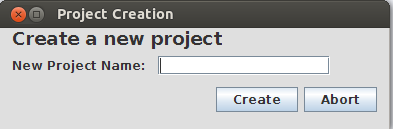
\includegraphics[width=\textwidth]{projCreate.png}
\caption{\textbf{Project creation dialog}}
\label{projCreate}
\end{figure}

\begin{figure}
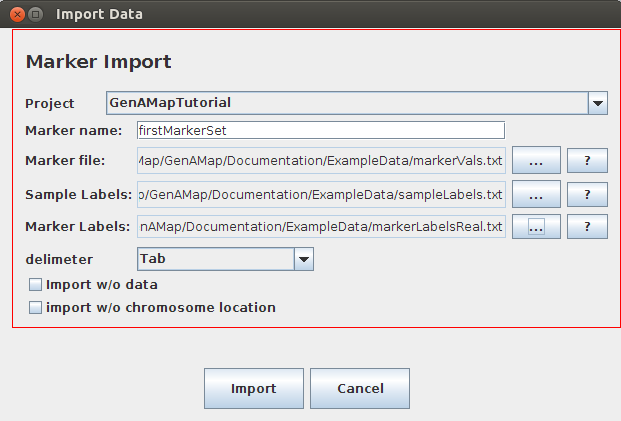
\includegraphics[width=\textwidth]{markerImport.png}
\caption{\textbf{Marker import dialog}}
\label{markerImport}
\end{figure}

\begin{figure}
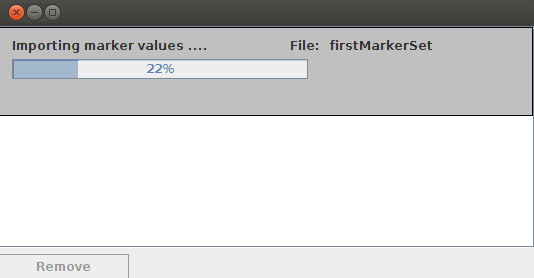
\includegraphics[width=\textwidth]{importBar.png}
\caption{\textbf{Data importing status bar}}
\label{importBar}
\end{figure}

\begin{figure}
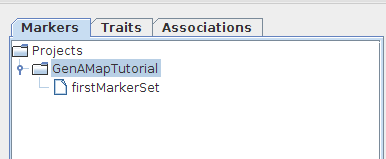
\includegraphics[width=\textwidth]{markerTabExample.png}
\caption{\textbf{Marker tab}}
\label{markerTab}
\end{figure}


\begin{figure}
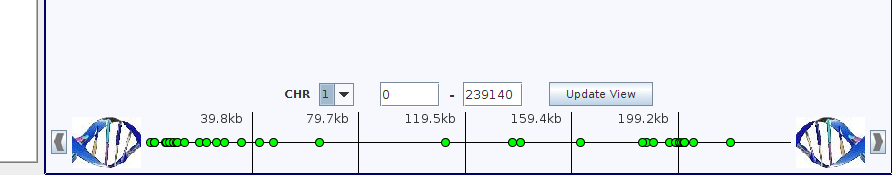
\includegraphics[width=\textwidth]{chromBrowser.png}
\caption{\textbf{Chromosome Browser}}
\label{chromBrowser}
\end{figure}


\begin{figure}
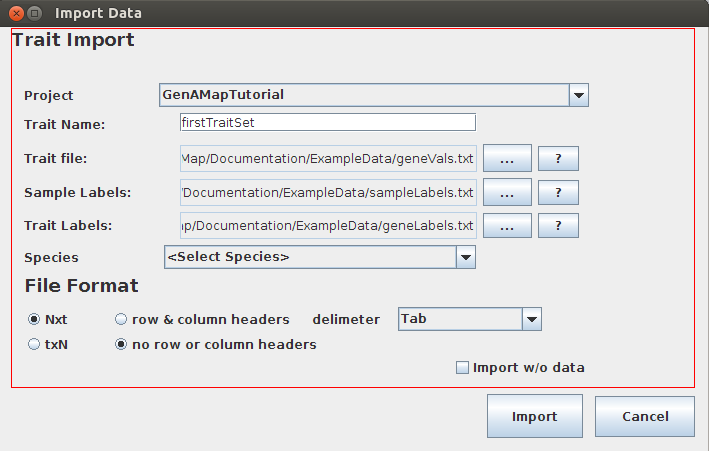
\includegraphics[width=\textwidth]{traitImport.png}
\caption{\textbf{Trait import dialog}}
\label{traitImport}
\end{figure}

\begin{figure}
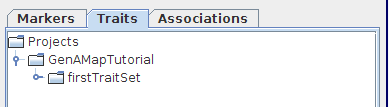
\includegraphics[width=\textwidth]{traitTabExample.png}
\caption{\textbf{Trait tab}}
\label{traitTab}
\end{figure}

\begin{figure}
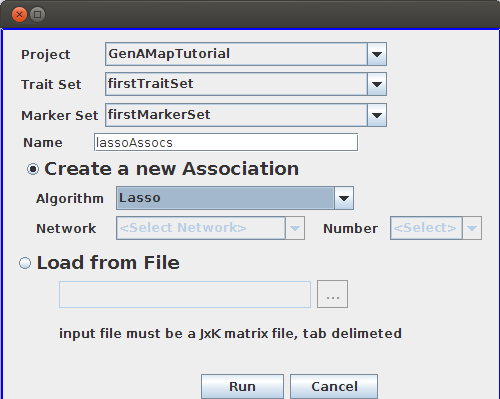
\includegraphics[width=\textwidth]{assocCreation.png}
\caption{\textbf{Association creation dialog}}
\label{assocCreation}
\end{figure}

\begin{figure}
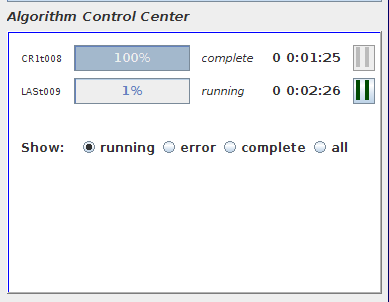
\includegraphics[width=\textwidth]{controlCenter.png}
\caption{\textbf{Algorithm Control Center}}
\label{controlCenter}
\end{figure}

\begin{figure}
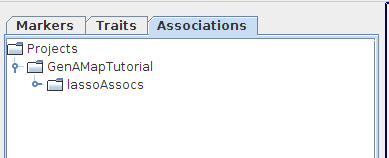
\includegraphics[width=\textwidth]{assocTab.png}
\caption{\textbf{Association Tab}}
\label{assocTab}
\end{figure}

\begin{figure}
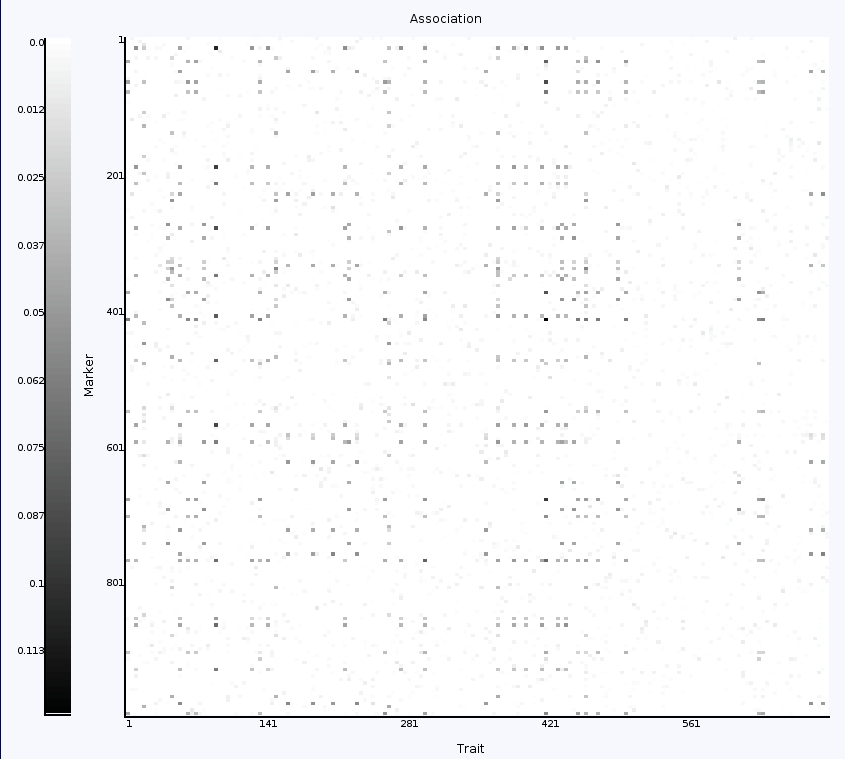
\includegraphics[width=\textwidth]{matrixView.png}
\caption{\textbf{Matrix View}}
\label{matrixView}
\end{figure}

\begin{figure}
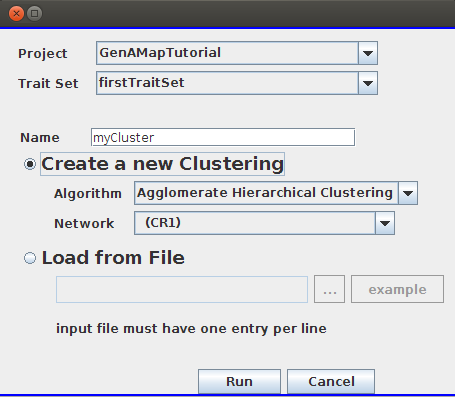
\includegraphics[width=\textwidth]{clusterCreation.png}
\caption{\textbf{Clustering creation dialog}}
\label{clusterCreation}
\end{figure}

\begin{figure}
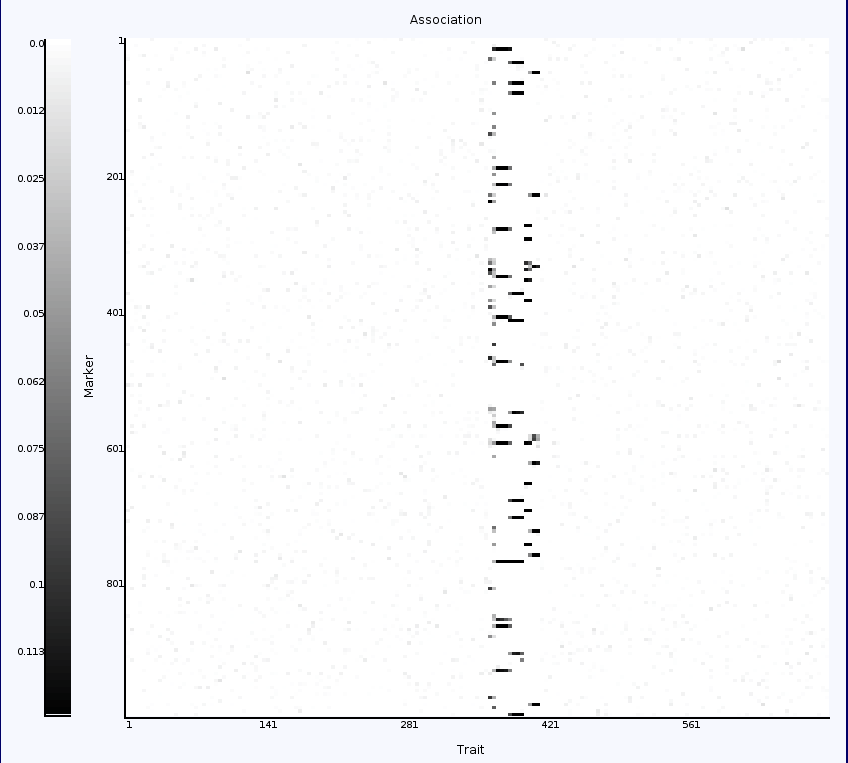
\includegraphics[width=\textwidth]{matrixViewClustered.png}
\caption{\textbf{Matrix View after applying Clustering}}
\label{matrixViewClustered}
\end{figure}

\begin{figure}
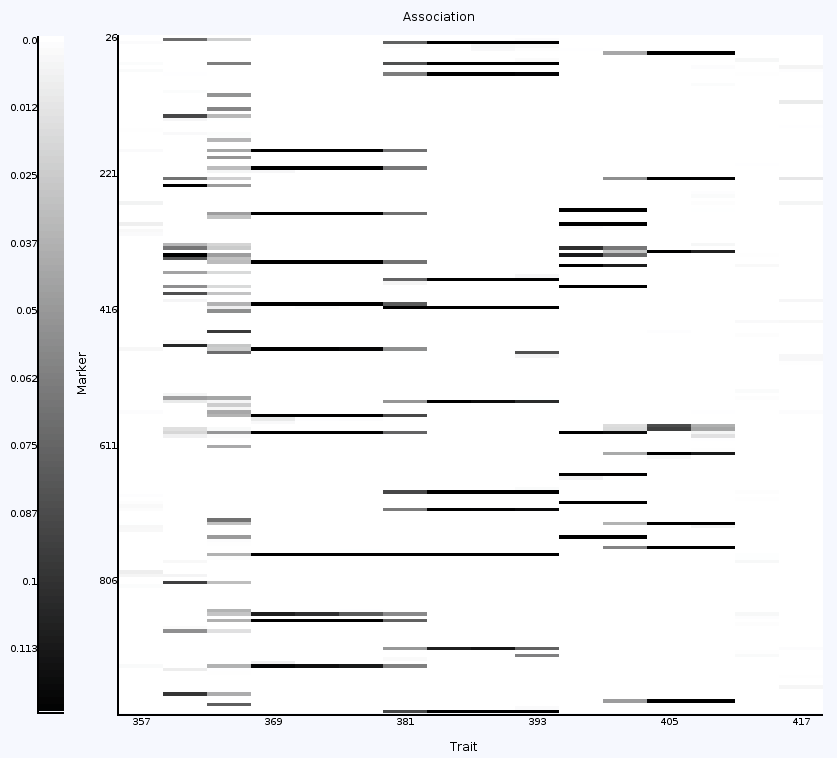
\includegraphics[width=\textwidth]{matrixViewZoomed.png}
\caption{\textbf{Matrix View after zooming}}
\label{matrixViewZoomed}
\end{figure}

\begin{figure}
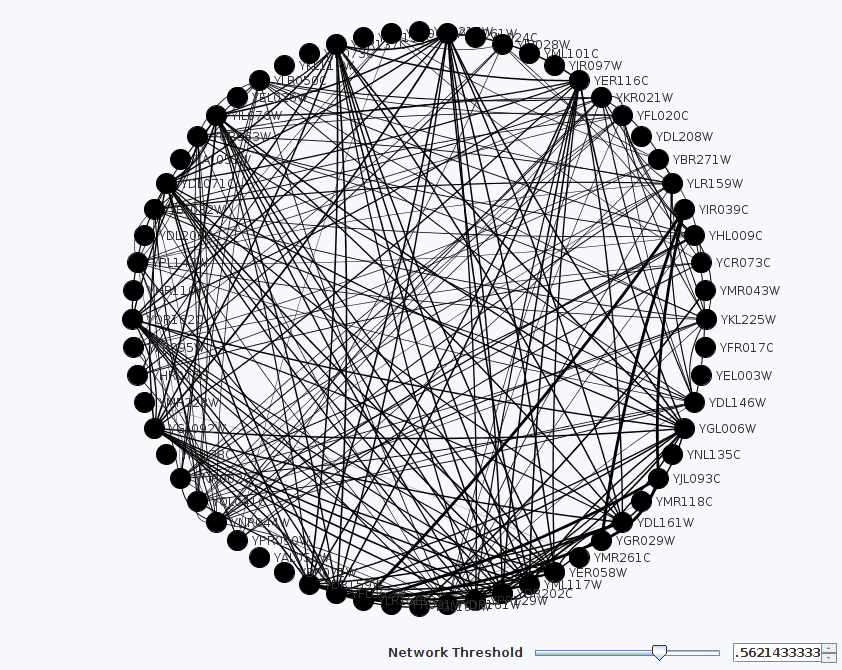
\includegraphics[width=\textwidth]{JUNG.png}
\caption{\textbf{JUNG View}}
\label{JUNG}
\end{figure}

\begin{figure}
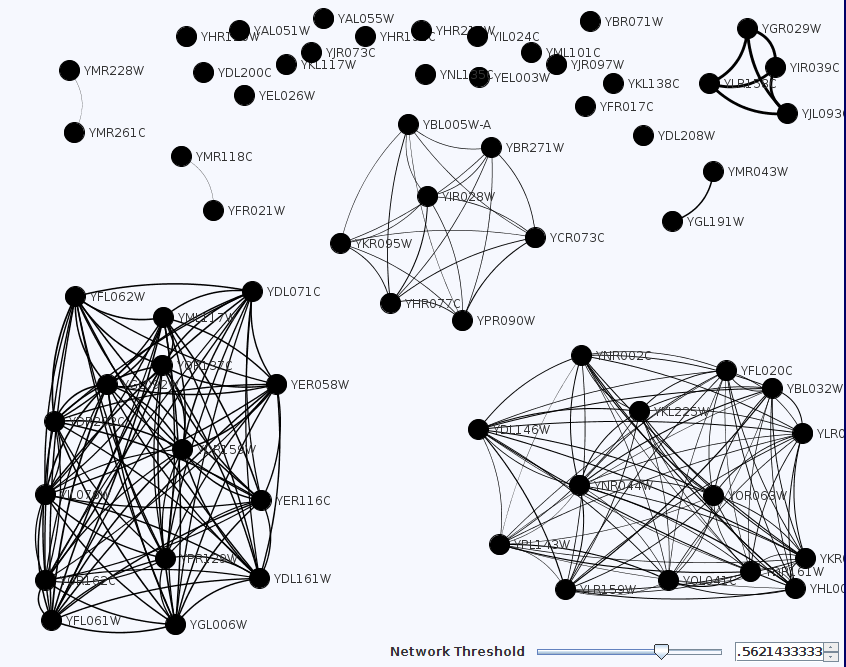
\includegraphics[width=\textwidth]{JUNGgrouped.png}
\caption{\textbf{JUNG View (user modified)}}
\label{JUNGgrouped}
\end{figure}

\begin{figure}
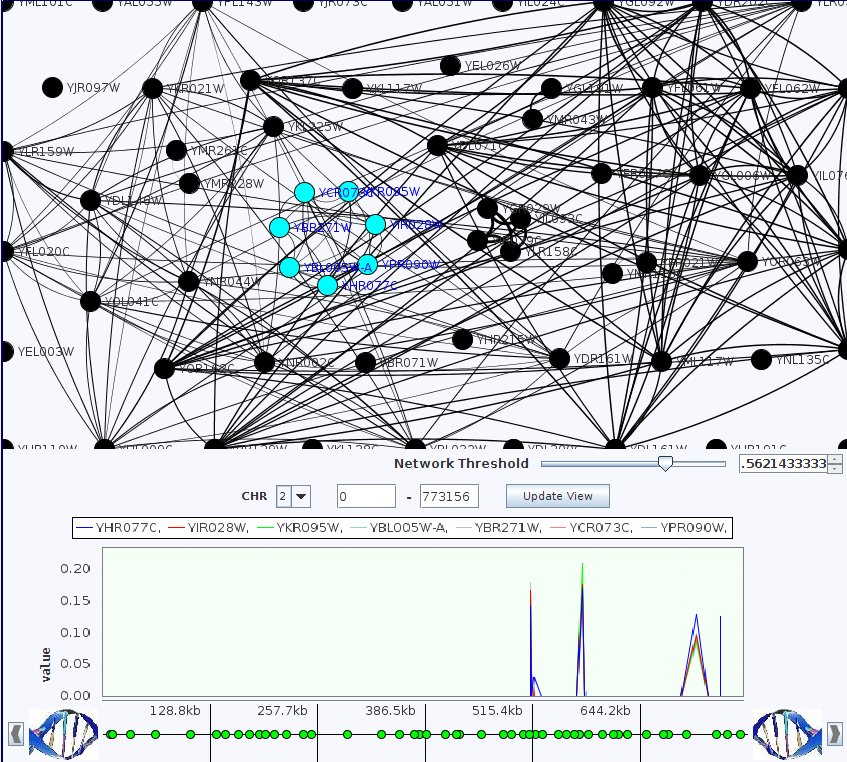
\includegraphics[width=\textwidth]{manhattan.png}
\caption{\textbf{Manhattan Plot}}
\label{manhattan}
\end{figure}


\pagebreak
\clearpage

\begin{figure}
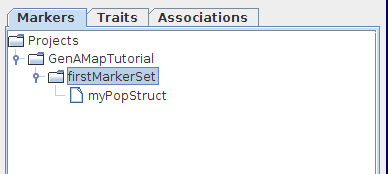
\includegraphics[width=\textwidth]{markerTab.png}
\caption{\textbf{Data organization in the Marker Tab}}
\label{markerTab}
\end{figure}

\begin{figure}
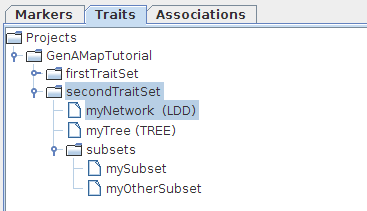
\includegraphics[width=\textwidth]{traitTab.png}
\caption{\textbf{Data organization in the Trait Tab}}
\label{traitTab}
\end{figure}

\begin{figure}
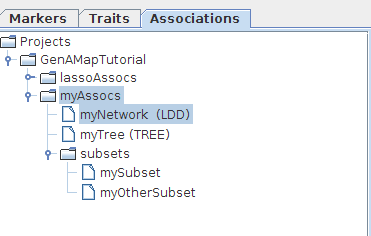
\includegraphics[width=\textwidth]{associationTab.png}
\caption{\textbf{Data organization in the Association Tab}}
\label{associationTab}
\end{figure}

\pagebreak
\clearpage

\begin{appendices}

\section{Video tutorials} \label{videos}

Below is a list of the video tutorials available on the GenAMap website (\url{http://sailing.cs.cmu.edu/genamap/tutorials.html}). %The red tags are the names of the video files in the GenAMap repository.

%Overview
\paragraph{GenAMap overview - bioVis 2011 video} is a walkthrough of the process of analyzing a dataset using the different visualization strategies available.
%MarkerImporting
\paragraph{Importing markers tutorial}  shows how Marker Data can be imported into GenAMap.
%ChromosomeView
\paragraph{Exploring and selecting markers tutorial} explains the Chromosome View, a visualization tool for Marker Data.
%PopulationStructureCreation / PopulationVisualization
\paragraph{Adding and viewing population structure tutorial} shows how we can add Population Structure data to a Marker Data set and the visualization options available for such data.
%AlgorithmControlCenter
\paragraph{Using the algorithm control center tutorial} details the options the user has to monitor and manage the algorithms that are running on the remote cluster.
%TraitImporting
\paragraph{Importing traits tutorial} shows how Trait Data can be imported into GenAMap.
%NetworkCreation
\paragraph{Adding network structure tutorial} explains the process of importing or using an algorithm to create a trait Network.
%Matrixview
\paragraph{How to use GenAMap's matrix view tutorial} exposes how to navigate the matrix view, one of the major visualization tools in GenAMap used for both Network Data and Association Data.
%Jungview
\paragraph{Network visualization using the JUNG view tutorial} demonstrates the features and capabilities of the JUNG view, one of the major visualization tools in GenAMap used for Network Data.
%ModuleCreation / ModuleVisualization
\paragraph{Gene module analysis tutorial} shows how to perform a Module Analysis (= create Module Data) as well as the options available for visualizing the results.
%SubsetCreation / SubsetVisualization
\paragraph{Trait subset overview tutorial} outlines the various options for creating Subset Data, as well as the various situations in which Subsets are created automatically by GenAMap.  
%TreeCreation
\paragraph{Adding tree data to trait data tutorial} details how Tree Data can be added either by importing or by creating it with an algorithm.
%TreeVisualization
\paragraph{Exploring trees overview tutorial} exposes the visualization tools available for exploring Trees.
%AssociationCreation
\paragraph{Running association algorithms tutorial} shows how to add Association Data to GenAMap, either by importing to by creating it with one of the available algorithms.
%AssociationVisualization
\paragraph{Association view overview tutorial} presents an overview of the core visualization tools for Association Data: the Matrix View, the JUNG View and the Chromosome Browser. This is done by following a realistic trajectory that data analysis might take in GenAMap.
%ManhattenPlot
\paragraph{Manhatten plots tutorial} presents the fourth and final major tool for visualizing Association Data: the Manhatten Plot.
%not yet available: AssociationComparison
%\paragraph{Using GenAMap to compare methods tutorial} shows several tools available for comparing different Association Data sets, which may be the result of analyses with different Association Algorithms.
%TraitFrequencyVisualization
\paragraph{Frequency tables and distribution analysis tutorial} introduces the Trait Frequency Table, which can be used to see how the distribution of specific traits differs as the marker value changes.
%PopulationVisualization2
\paragraph{Population association analysis visualizations tutorial} shows how we can explore results from Association Algorithms that use Population Structure as input. These algorithms produce different results for each population in the Marker Data set.
%WebInterface
\paragraph{Links to outside databases tutorial} presents GenAMap's capabilities to link directly to external resources dbSNP, SGD, UniProt and Google Search.
%ThreewayCreation
\paragraph{How to add a three-way visualization tutorial} shows how to run gGfLasso, the algorithm used to create 3-way association data. 
%FeatureLoading
\paragraph{Running AMTL and uploading SNP features} explains how to import Feature Data, which contains quantitative information about markers and can be used to run the AMTL algorithm.
%ThreewayVisualization
\paragraph{Three way visualization tutorial} is a set of three detailed videos about GenAMap's extensive capabilities for visualizing 3-way association data.

\section{Data Types} \label{types}

\begin{longtable}{p{2cm}p{4cm}p{4cm}p{2cm}p{2cm}}
\hline Name&Description&Format&References&Action \\  \hline

\endhead

Marker Data & Marker values of samples & Numerical matrix & - & load \\ \hline
Trait Data & Trait values of samples & Numerical matrix & - & load \\ \hline
Network & Relatedness of traits & Square, symmetric numerical matrix & Trait Data set & load \& create \\ \hline
Association Data & Associations between markers and traits & Numerical matrix & Marker \& Trait Data set & load \& create \\ \hline
Clustering & Trait permutation that induces grouping by relatedness & List of trait indices & Trait Data set & load \& create \\ \hline
Tree & Tree structure over traits capturing relatedness & Linked list of traits & Trait Data set & load \& create \\ \hline
Subset & Subset of traits in a Trait Data set & List of traits & Trait Data set & load \& create \\ \hline
Module Data & Subsets of traits with GO and eQTL annotation & Lists of traits with GO / eQTL table & Trait Data set \& Clustering & create \\ \hline
Population Structure & Clustering of samples in Marker Data set & Lists of samples & Marker Data set & load \& create \\ \hline
Feature & Quantitative annotation for markers & Numerical vector & Marker Data set & load \\ \hline
3way Association Data & Associations between markers, gene expression traits and phenotypic traits & Numerical matrix & Association Data set & create \\ \hline

\end{longtable}


\section{Visualization Tools} \label{visTools}

\begin{longtable}{p{4cm}p{6cm}p{4cm}}
\hline Name & Description & Applicable Data Types\\  \hline
Chromosome Browser & Viewing the location of markers on the chromosome&Marker Data\\  \hline
Matrix View & Visual representation of trait value matrix and association value matrix&Network \& Association Data\\  \hline
JUNG View & Ball-and-stick representation of trait network & Network \\  \hline
Manhattan Plot & Plotting the associations of selected traits against the genome & Association Data \\  \hline
Tree View & Exploring a trait Tree & Tree\\  \hline
3way Visualization & Ball-and-stick representation of 3way Association Data & 3way Association Data\\  \hline
Population Structure View & Plots of samples by population & Population Structure\\  \hline
Trait Frequency View & Histogram of trait values by marker value & Association Data\\  \hline
\end{longtable}

\section{Web-Based External Resources} \label{resources}

\begin{longtable}{p{4cm}p{4cm}p{4cm}}
\hline Name of Database&Searchable Entity&Required Entity Name \\  \hline

\endhead

Saccharomyces Genome Database (SGD) & Marker & Gene name \\ \hline
dbSNP & Marker & rs\# \\ \hline
Google & Trait & various \\ \hline
UniProt & Trait & Gene name \\ \hline

\end{longtable}




\end{appendices}





\end{document}